% % % % % % % % % % % % % % % % % % % % % % % % % % % % % % % % % % % % % % % % % % % %
%                                                                                     %
% Short Sectioned Assignment LaTeX Template Version 1.0 (5/5/12)                      %
% This template has been downloaded from: http://www.LaTeXTemplates.com               %
%                                                                                     %
% Original author:  Frits Wenneker (http://www.howtotex.com)                          %
%                                                                                     %
% Modified by: Fco Javier Sueza Rodríguez (fcosueza@disroot.org)                      %
%                                                                                     %
% Changes:                                                                            %
%	    - Custom Chapters, Sections and Subsections (titlesec package)                %
%           - Document type scrbook (oneside)                                         %
%           - Use babel-lang-spanish package and marvosym                             %
%           - Use hyperref, enumitem, tcolorbox and glossaries packages               %
%           - Use Time New Roman (mathptmx), Helvetic and Courier fonts               %
%                                                                                     %
% License: CC BY-NC-SA 3.0 (http://creativecommons.org/licenses/by-nc-sa/3.0/)        %
%                                                                                     %
% % % % % % % % % % % % % % % % % % % % % % % % % % % % % % % % % % % % % % % % % % % %

%-----------------------------------------------%
%	              Packages                  %
%-----------------------------------------------%

\documentclass[paper=a4, fontsize=11pt, oneside]{scrbook}

% ---- Text Input/Output ----- %

\usepackage[T1]{fontenc}
\usepackage[utf8]{inputenc}
\usepackage{mathptmx}
\usepackage[scaled=.92]{helvet}
\usepackage{courier}
\usepackage[indent=12pt]{parskip}

\usepackage{geometry}
\geometry{verbose,tmargin=3cm,bmargin=3cm,lmargin=2.6cm,rmargin=2.6cm}

% ---- Language ----- %

\usepackage[spanish]{babel}
\usepackage{marvosym}

% ---- Another packages ---- %

\usepackage{amsmath,amsfonts,amsthm}
\usepackage{graphics,graphicx}
\usepackage{titlesec}
\usepackage{fancyhdr}
\usepackage{tcolorbox}
\usepackage{hyperref}
\usepackage{enumitem}
\usepackage[automake]{glossaries}

%--------------------------------------------------------------------%
%                      Customizing Document                          %
%--------------------------------------------------------------------%


% ----------- Custom Chapters, Sections and Subsections -------------- %

\titleformat{\chapter}[display]
			{\bfseries\Huge}
			{Tema \ \thechapter} {0.5ex}
			{\vspace{1ex}\centering}

\titleformat{\section}[hang]
			{\bfseries\Large}
			{\thesection}{0.5em}{}

\titleformat{\subsection}[hang]
			{\bfseries\large}
			{\thesubsection}{0.5em}{}

\titleformat{\subsubsection}[hang]
			{\bfseries\large}
			{\thesubsubsection}{0.5em}{}

\hypersetup{
    colorlinks=true,
    linkcolor=black,
    urlcolor=magenta
}

% ------------------- Custom heaaders and footers ------------------- %

\pagestyle{fancyplain}

\fancyhead[]{}
\fancyfoot[L]{}
\fancyfoot[C]{}
\fancyfoot[R]{\thepage}

\renewcommand{\headrulewidth}{0pt} % Remove header underlines
\renewcommand{\footrulewidth}{0pt} % Remove footer underlines

\setlength{\headheight}{13.6pt} % Customize the height of the header

% --------- Numbering equations, figures and tables ----------------- %

\numberwithin{equation}{section} % Number equations within sections
\numberwithin{figure}{section} % Number figures within sections
\numberwithin{table}{section} % Number tables within sections

% ------------------------ New Commands ----------------------------- %

\newcommand{\horrule}[1]{\rule{\linewidth}{#1}} % Create horizontal rule command


%----------------------------------------------------------------------------------------
%	TÍTULO Y DATOS DEL ALUMNO
%----------------------------------------------------------------------------------------

\title{
\vspace{10ex}
\normalfont \normalsize
\huge \textbf{Instalación y Administración de Servidores de Ficheros de Alta Disponibilidad}
}
\author{Francisco Javier Sueza Rodríguez}
\date{\normalsize\today}

%----------------------------------------------------------------------------------------
%                                     DOCUMENTO
%----------------------------------------------------------------------------------------
\begin{document}


\maketitle

\thispagestyle{empty}

\vspace{65ex}

\begin{center}
    \begin{tabular}{l l}
        \textbf{Centro}: & IES Aguadulce \\
        \textbf{Ciclo Formativo}: & Desarrollo Aplicaciones Web (Distancia)\\
        \textbf{Asignatura}: & Despliegue de Aplicaciones Web\\
        \textbf{Tema}: & Tema 3 - Instalación y Administración de Servidores de Ficheros de Alta Disponibilidad\\
    \end{tabular}
\end{center}

\newpage

\tableofcontents

\newpage

\listoffigures

\newpage


\section{Introducción}
En este bloque de actividades vamos a realizar la instalación y configuración del servicio FTP tanto a nivel de servidor como de cliente, sobre un servidor \textbf{Linux Ubuntu 14/16/18/20/22} (Se admite Debian 9/10/11). A continuación enumero los distintos apartados de la práctica.

\section{Ejercicios}

\subsection{Ejercicio 1: Instalación de un servidor FTP}
Realiza la instalación del servidor \textbf{FTP ProFTPd} en tu servidor Ubuntu/Debian desde el repositorio, comprobando su funcionamiento e indicando cómo se inicia y cómo se para, cómo se comprueba su estado y localiza en el fichero de configuración la línea en la que especifica que se ha instalado en \textbf{modo ``standalone''}. Documenta el proceso de instalación, explica porque hemos elegido que se ejecute como un \textbf{servidor independiente} y comprueba el funcionamiento conectándote desde la consola de comandos con tu usuario de sistema.

\subsubsection{Solución}
Para realizar la instalación de ProFTPd se va a usar el gestor de paquetes de Ubuntu, APT, usando el comando \textbf{\textit{apt-get install proftpd}}, que realizará una instalación del servidor ftp. El servidor se instala por defecto en modo \textbf{standalone}, por lo que no habrá que modificar nada para instalarlo en esta modalidad.

En la siguiente imagen vemos la ejecución del comando APT y la instalación del paquete.

\begin{figure}[H]
    \centering
    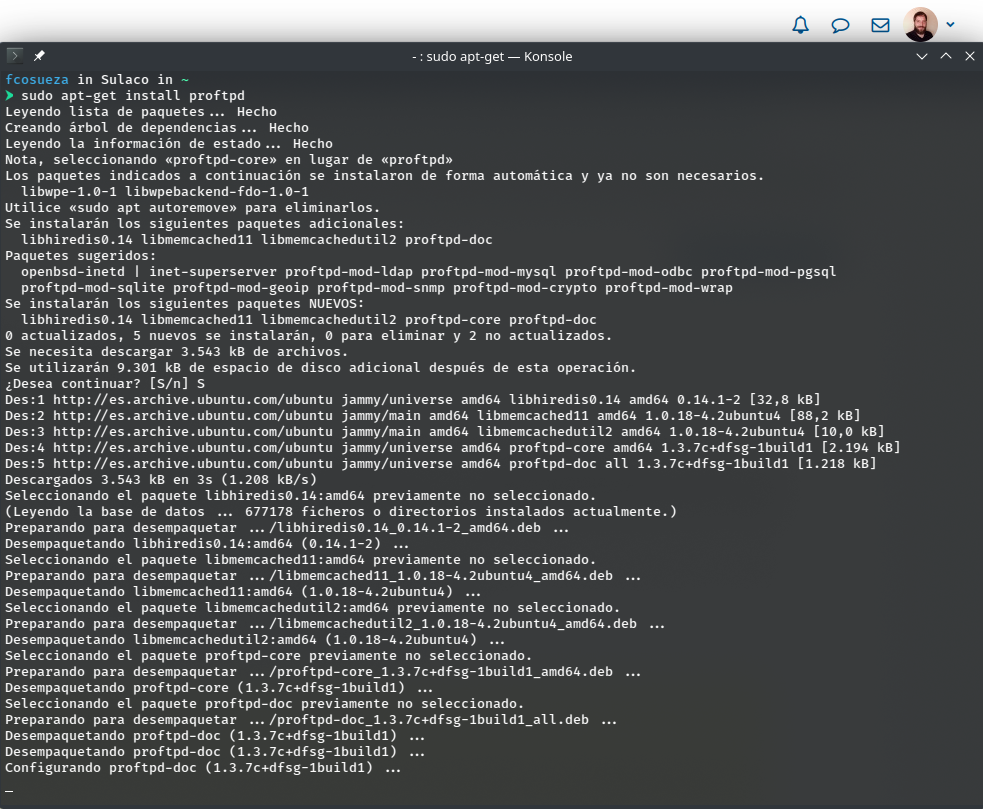
\includegraphics[scale=0.51]{instalacion.png}
    \caption{Instalación de ProFTPd mediante APT}
\end{figure}

En el \textbf{modo standalone}, es el servidor el que esta escuchando en el puerto por defecto y el que procesa las conexiones, evitando crear un proceso nuevo con cada conexión, ya que mediante inetd es este servicio el que escucha en el puerto y con cada conexión crea una instancia de proftpd.

En Ubuntu, para iniciar y parar el servidor se puede usar el comando \textbf{\textit{service}}, usándolo con los parámetros oportunos, por ejemplo \textbf{\textit{service proftpd start}} y \textbf{\textit{service proftpd stop}}, para iniciarlo y detenerlo respectivamente, como podemos ver en la siguiente captura.

\begin{figure}[H]
    \centering
    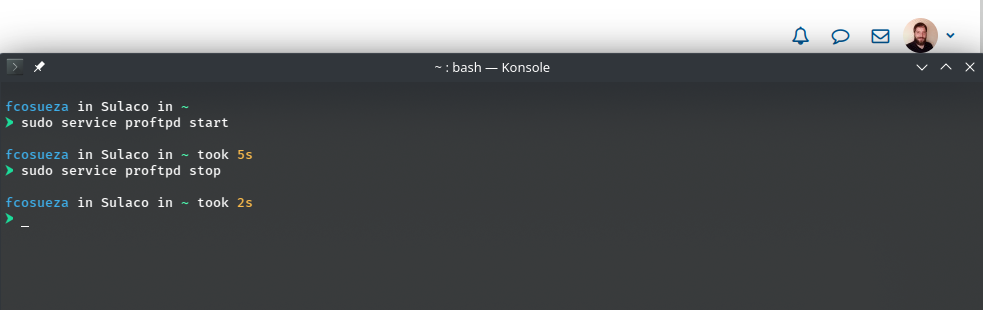
\includegraphics[scale=0.55]{inicio-parada.png}
    \caption{Inicio y parada del servidor usando service}
\end{figure}

Para comprobar que se ha realizado la instalación e inicialización correctamente, se ha realizado una conexión desde consola, usando nuestro usuario del sistema, mediante el comando \textbf{\textit{ftp 127.0.0.1}}. En la siguiente imagen, se puede ver como se ha realizado la conexión y se ha usado el comando ls.

\begin{figure}[H]Configura ProFTPd para que enjaule a los usuarios anónimos en esta carpeta y no les permita escribir ni modificar los archivos, solo descargar.
    \centering
    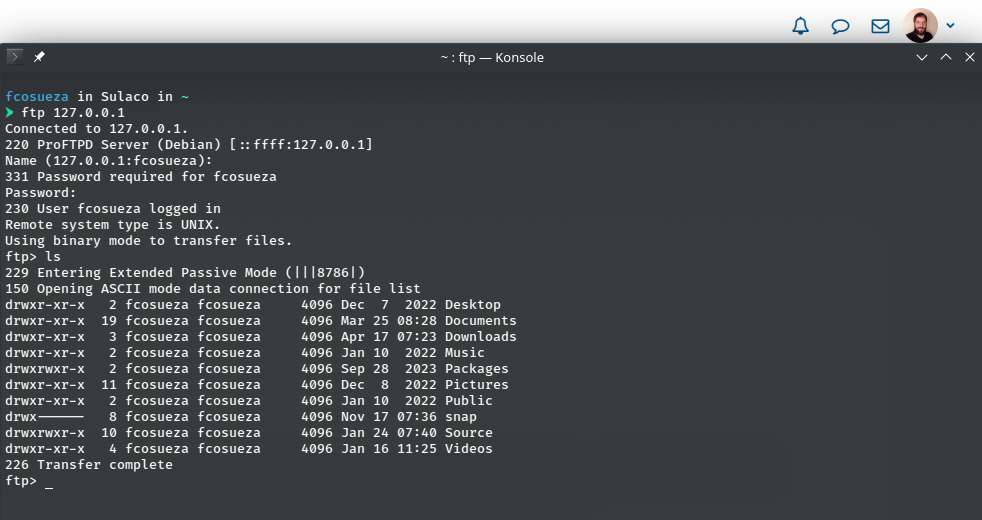
\includegraphics[scale=0.55]{conexion.png}
    \caption{Conexión al servidor FTP}
\end{figure}

\subsection{Ejercicio 2: Configurar el acceso anónimo para el servidor FTP}
En esta actividad debemos configurar el servidor ProFTPd para que permita el acceso de \textbf{usuarios anónimos}, realizando las siguientes tareas:

\begin{itemize}
    \item Crea una carpeta con la ruta /var/ftp/distancia y dentro de ella un fichero de texto cuyo nombre será anonymous.txt.
    \item Configura ProFTPd para que enjaule a los usuarios anónimos en esta carpeta y no les permita escribir ni modificar los archivos, solo descargar.
    \item Ajusta los parámetros del servidor FTP para que permita 40 conexiones simultáneas de usuarios anónimos.
    \item Una vez configurado, conéctate con el usuario anónimo y comprueba que tienes acceso al fichero, utilizando el cliente FTP incluido en Linux desde la consola de comandos.
\end{itemize}

\subsubsection{Solución}
En este ejercicio vamos a configurar el servidor para que acepte conexiones de usuario anónimos. En primer lugar, hemos creado la carpeta \textbf{\textit{/var/ftp/distancia}}, que será la que usaremos como directorio raíz para los usuarios anónimos. En la siguiente captura se puede ver la creación de la carpeta.

\begin{figure}[H]
    \centering
    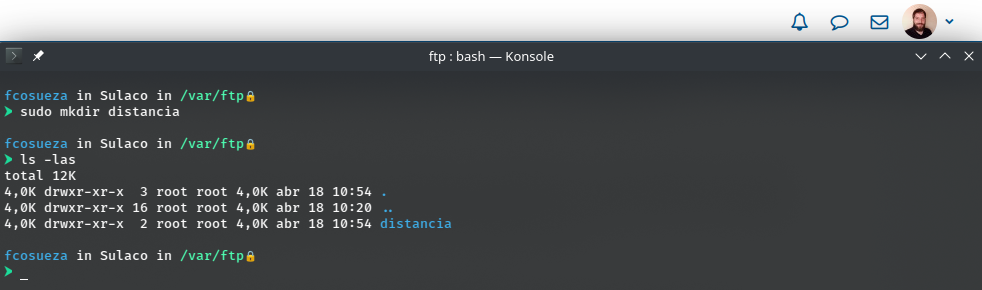
\includegraphics[scale=0.55]{carpeta.png}
    \caption{Creación de la carpeta para los usuarios anónimos}
\end{figure}

El siguiente paso es \textbf{configurar Proftpd} para que cambie la raíz de los usuarios anónimos a esta carpeta y que además no les permita ni escribir ni modificar archivos, solo descargarlos.

En el \textbf{archivo de configuración} por defecto de proftpd ya viene una \textbf{configuración básica} para permitir el acceso anónimo. Esta configuración suele venir comentada en el fichero, así que solo tendremos que descomentar las opciones y modificar las que nos interesen, ya que la configuración que viene por defecto es bastante completa.

En este caso, se han realizado unas mínimas modificaciones en la configuración por defecto que proporciona ProFTPd. En primer lugar, se ha cambiado el número máximo de conexiones anónimas permitidas a 40, cambiando al directiva \textbf{\textit{MaxClients}}. Además, se ha cambiado el directorio por defecto de los usuarios anónimos, añadiéndole el directorio creado en este punto a la directiva \textbf{\textit{<Anonymous>}}. También se le ha cambiado el nombre al servidor a \textbf{Despliegue de Aplicaciones}.

En la siguiente captura podemos ver la sección de la configuración que hemos modificado para el servidor anónimo.

\begin{figure}[H]
    \centering
    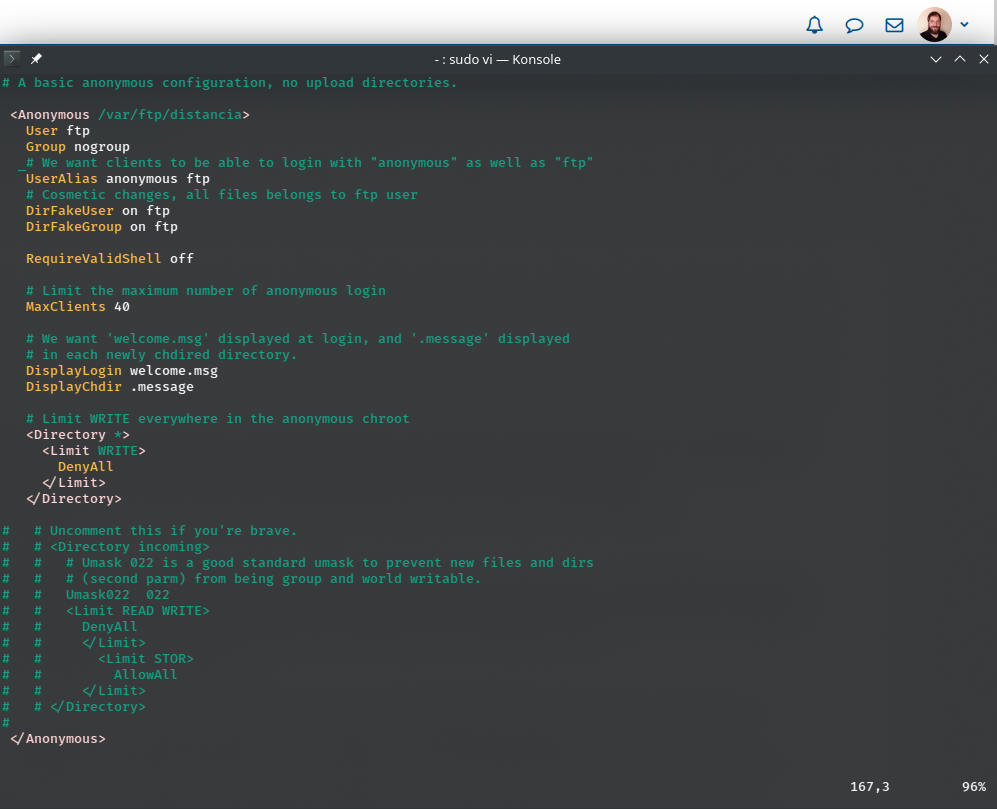
\includegraphics[scale=0.55]{ftp-anon.png}
    \caption{Configuración para el FTP anónimo en ProFTPd}
\end{figure}

Una vez configurado el servidor, se ha reiniciado el servidor con el comando \textbf{\textit{service proftpd restart}} y se ha comprobado que se puede conectar como anónimo, así como las restricciones de permisos.

\begin{figure}[H]
    \centering
    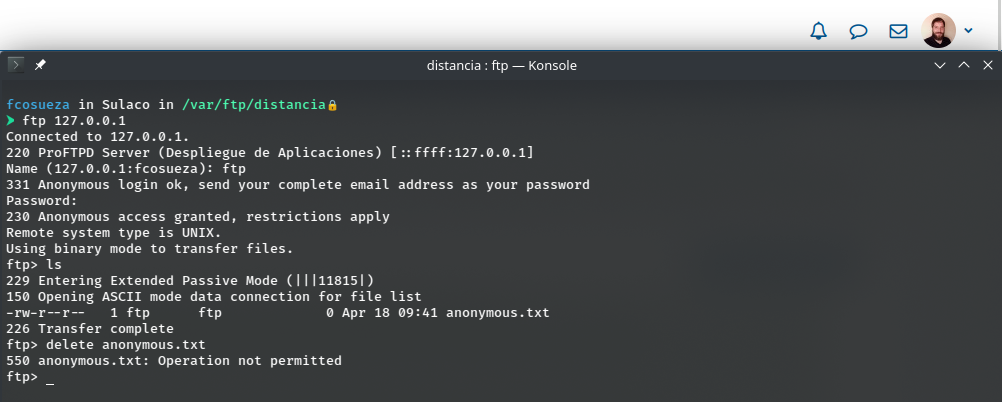
\includegraphics[scale=0.55]{ftp-anon-check.png}
    \caption{Configuración para el FTP anónimo en ProFTPd}
\end{figure}

\subsection{Ejercicio 3: Creación de un usuario virtual}
Configura el servidor ProFTPd para que se pueda acceder mediante usuarios virtuales, teniendo en cuenta lo siguiente:

\begin{itemize}
    \item Crea un usuario virtual con el nombre 'vdawXXX' donde XXX son los 3 últimos dígitos de tu DNI.
    \item El fichero que contiene los usuarios estará en la carpeta /etc/proftpd/distancia/
    \item La carpeta que se asignará a este usuario al conectarse estará en /var/ftp/vdawXXX
    \item Recuerda comprobar los permisos de esta carpeta para que pueda gestionarla el usuario que ejecuta el servicio FTP.
    \item Una vez configurado, conéctate con el usuario virtual desde la consola de comandos y comprueba que puedes subir un fichero.
\end{itemize}

\subsubsection{Solución}
En este ejercicio vamos a crear un usuario virtual haciendo uso del comando \textbf{ftpasswd}, que vamos a describir paso a paso.

En primer lugar, vamos a crear las carpetas \textbf{/etc/proftpd/distancia/} y \textbf{/var/ftp/vdaw618} como se especifica en el enunciado. La primera albergará los archivos de login del usuario y la segunda será su carpeta home.  En la siguiente captura, podemos ver la creación de ambos directorios.

\begin{figure}[H]
    \centering
    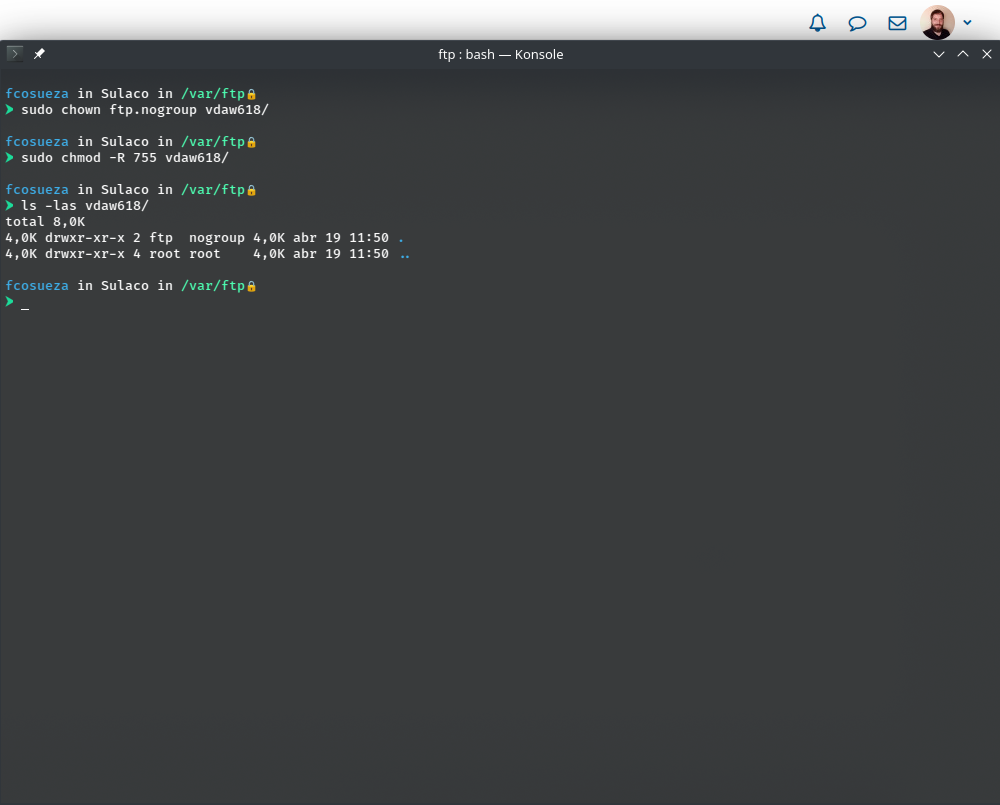
\includegraphics[scale=0.50]{virtual-1.png}
    \caption{Creación de las carpetas para el usuario virtual}
\end{figure}

Una vez que hemos creado las carpetas, deberemos\textbf{ cambiar los permisos} del directorio \textbf{/var/ftp/vdaw618} para que no se creen conflictos con el usuario. Para ello, usaremos el comando \textit{\textbf{chown}}, estableciendo el usuario a \textbf{ftp} y el grupo a \textbf{nogroup}. Además, otorgaremos permisos de lectura, escritura y ejecución al usuario en dicha carpeta y de lectura y ejecución al resto de usuarios, con \textbf{chmod}, como podemos ver en la siguiente captura.
\begin{figure}[H]
    \centering
    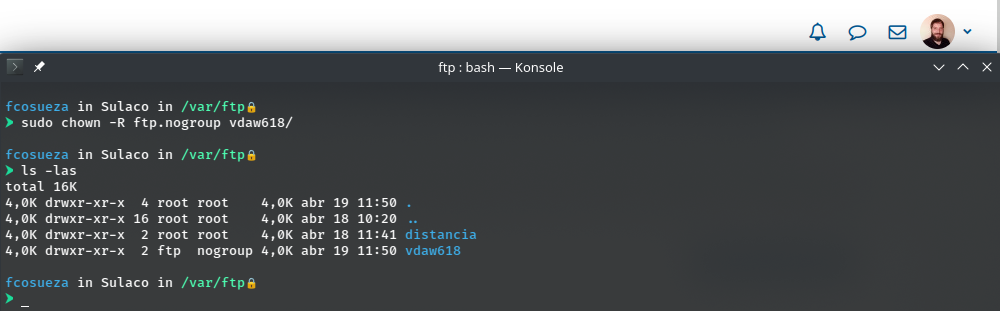
\includegraphics[scale=0.50]{virtual-2.png}
    \caption{Cambio de los permisos en la carpeta raíz del usuario virtual}
\end{figure}

El siguiente paso es crear el usuario con el comando \textbf{ftpasswd}. En la siguiente captura vemos la ejecución de este comando, y ahora pasaremos a explicar los parámetros que le hemos pasado.

\begin{figure}[H]
    \centering
    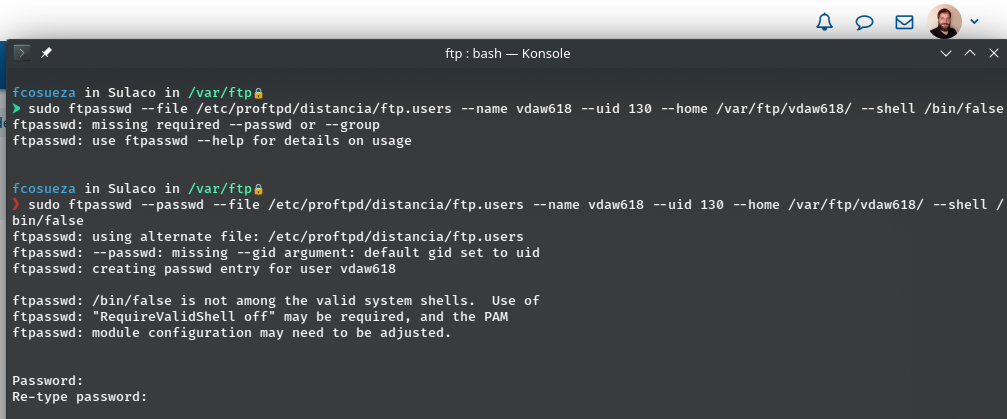
\includegraphics[scale=0.50]{virtual-3.png}
    \caption{Creación del usuario con ftpasswd}
\end{figure}

Durante el proceso de creación, se nos pedirá la contraseña, que insertaremos y el usuario será creado. Los parámetros que se le han pasado al comando son los siguientes:

\begin{itemize}
    \item \textbf{--passwd}: especifica que se tiene que pedir una contraseña para el usuario durante el proceso de creación.
    \item \textbf{--file /etc/proftpd/distancia/ftp.users}: este parámetro especifica el fichero donde se guardará la información del usuario virtual.
    \item \textbf{--name vdaw618}: le indicamos que el nombre del usuario va ser vdaw618.
    \item \textbf{--uid 130}: indicamos con el UID se creará el usuario. Podemos indicarle cualquiera, aunque no debemos nunca indicarle el UID 0, ya que es el del usuario root y puede suponer un grave problema de seguridad. Aquí se le ha asignado el del usuario ftp, que es el 130. Puede que en otros sistemas el UID de ftp sea diferente, pero podemos consultarlo en el archivo /etc/passwd.
    \item \textbf{--home /var/ftp/vdaw618/}: indicamos cual será el directorio raíz de este usuario.
    \item \textbf{--shell /bin/false}: con este comando se le indica que shell usará el usuario. Indicandole que use /bin/false, no se le permitirá acceder a la shell del sistema, evitando posibles problemas de seguridad.
\end{itemize}

Por último, hemos \textbf{modificado el archivo de configuración} de ProFTPd y añadido dos líneas para especificar el fichero donde están los usuarios virtuales y que no se requiera una shell válida para su conexión, como vemos en la siguiente captura.

\begin{figure}[H]
    \centering
    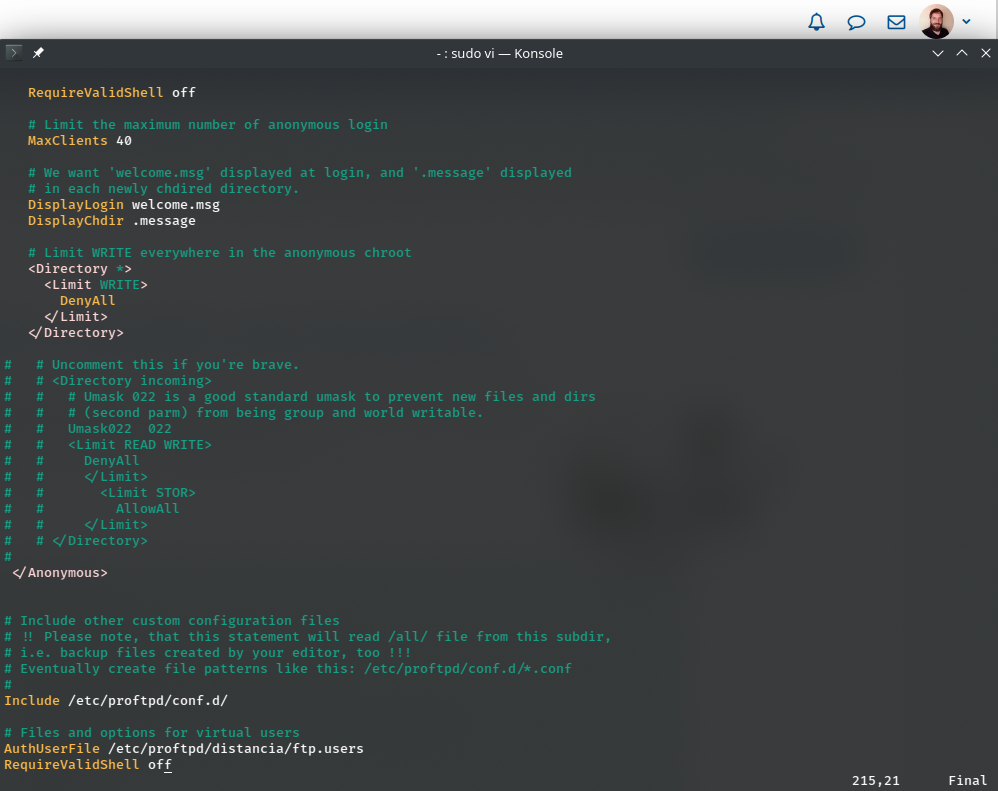
\includegraphics[scale=0.45]{virtual-4.png}
    \caption{Modificación del fichero de configuración de ProFTPd}
\end{figure}


Por último, comprobamos que se ha creado el usuario correctamente. Para ello hemos conectado al ftp empleando el usuario y la contraseña que hemos creado como credenciales y se ha subido el archivo prueba.txt. Todo se ha realizado correctamente, como vemos en la siguiente captura.

\begin{figure}[H]
    \centering
    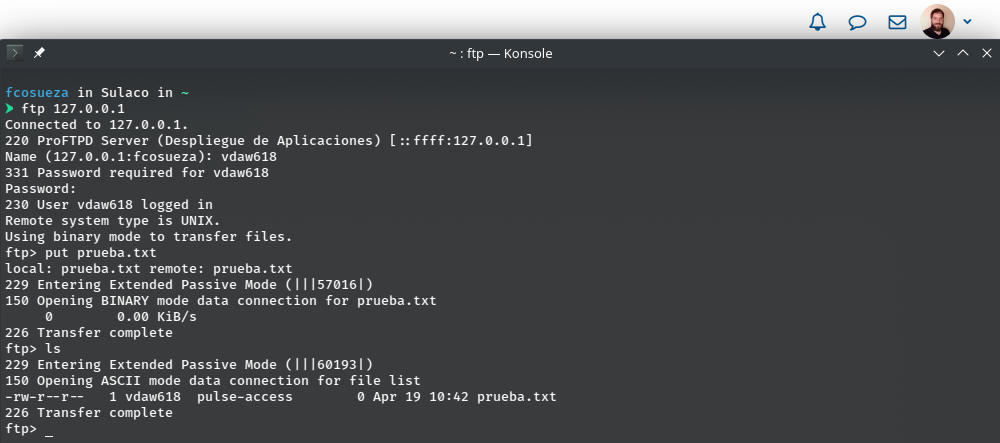
\includegraphics[scale=0.45]{virtual-5.png}
    \caption{Comprobación de que se ha creado correctamente}
\end{figure}

\subsection{Ejercicio 4: Configuración del servidor FTP para conexión segura con TSL}
Configura el servidor FTP para que acepte conexiones seguras (TLS), teniendo en cuenta lo siguiente:

\begin{itemize}
    \item Crea/Instala un certificado en tu servidor Ubuntu/Debian
    \item Modifica los ficheros de configuración para que utilicen este certificado.
    \item Configura el servidor para que el usuario creado en la actividad 3 pueda conectarse mediante esta conexión cifrada.
    \item Debes documentar tanto la creación del certificado como la modificación de los ficheros de configuración.
    \item Una vez configurado, conéctate con el usuario virtual desde la consola de comandos y comprueba que puedes subir un fichero.
\end{itemize}

\subsubsection{Solución}
En este ejercicio vamos a configurar el servidor ProFTPd para que pueda realizar conexiones seguras mediante el uso de TLS.  Para ello, vamos a crear un certificado usando utilizad que proporciona el servidor, \textbf{proftpd-gencert}, ya que es mucho más rápido y cómodo, con el único ``inconveniente'' de que el certificado creado será válido solo durante un año, que tampoco está nada mal.

En primer lugar hemos \textbf{descomentado la línea} en la configuración de ProFTPd para que se incluya el fichero de configuración
\textbf{\textit{/etc/proftpd/tsl.conf}}, como podemos ver en la siguiente captura.

\begin{figure}[H]
    \centering
    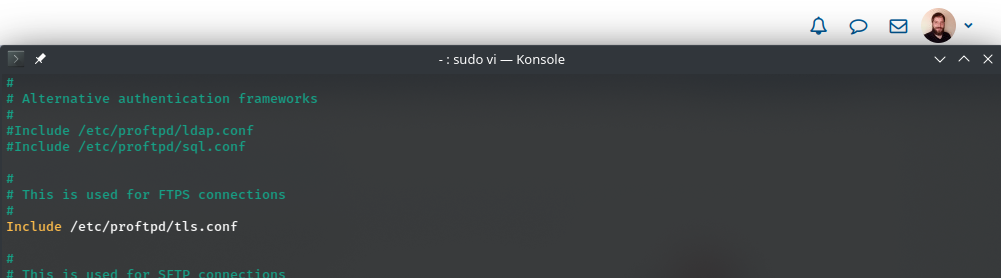
\includegraphics[scale=0.55]{tsl-1.png}
    \caption{Inclusión del archivo tsl.conf en la configuración de ProFTPd}
\end{figure}

El siguiente paso, es usar el comando \textbf{proftpd-gencert} para generar la claves privada y pública para poder cifrar la conexión. Durante la ejecución del este comando, se nos pedirá varios datos, como la abreviatura de nuestro país, localidad, nombre de nuestra empresa, nuestros nombre, etc.

Una vez rellenados todos los datos que nos pidan, se generarán dos ficheros con los certificados SSL, en concreto, un fichero con el certificado en \textbf{\textit{/etc/ssl/certs/proftpd.crt}} y otro con la llave SSL en \textbf{\textit{/etc/ssl/private/proftpd.key
}}. En el siguiente paso, cambiaremos los permisos de estos archivos y moveremos la llave al directorio de SSL.

Este proceso también se podría haber realizado instalando \textbf{openssly}  y usando el comando \textbf{openssl}, pero nos has parecido más rápido y cómodo hacerlo usando la aplicación que ya incorpora ProFTPd.

En la siguiente captura podemos ver la generación de las claves con el comando proftpd-gencert.

\begin{figure}[H]
    \centering
    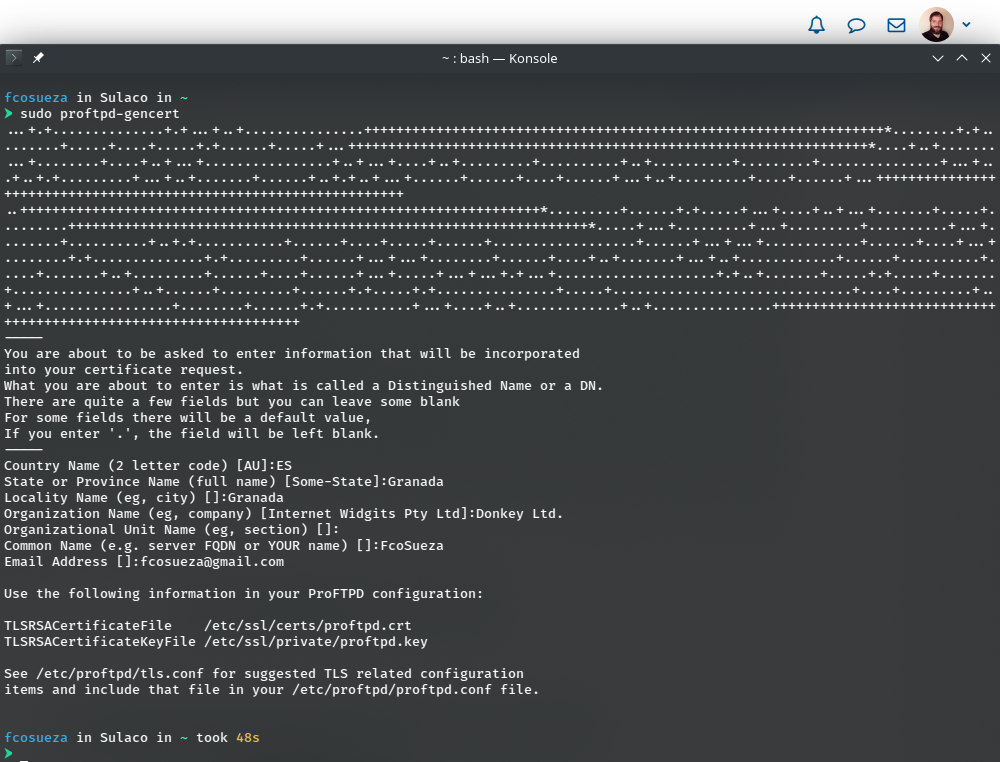
\includegraphics[scale=0.50]{tsl-2.png}
    \caption{Inclusión del archivo tsl.conf en la configuración de ProFTPd}
\end{figure}

El siguiente paso es mover la llave generada al directorio de SSL en \textit{\textbf{/etc/ssl/}} además de cambiarles los permisos a los archivos generados. En la siguiente captura, vemos como se ha llevado a cabo esta acción y los permisos que se han establecido en ambos ficheros.

\begin{figure}[H]
    \centering
    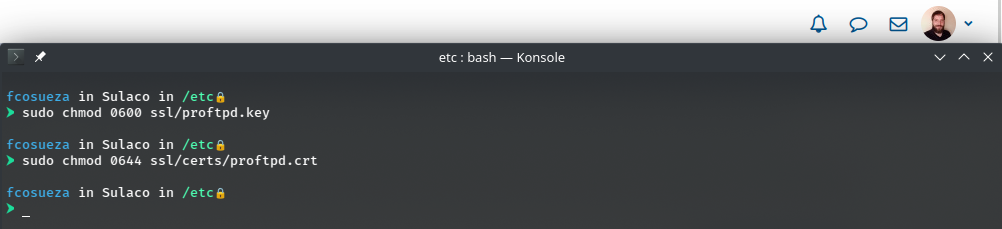
\includegraphics[scale=0.50]{tsl-3.png}
    \caption{Cambio de permisos de los archivos generados}
\end{figure}

Por último, se ha modificado el fichero \textbf{\textit{/etc/proftpd/tls.conf}}, donde se encuentra la configuración del servidor para TLS.

El resultado es que se han modificado pocas opciones, en su mayoría solo se han descomentado, ya que la configuración por defecto que ofrece ProFTPd para la conexión segura FTPS se ha adaptado bastante bien a nuestros requisitos.

Una de las opciones que si se ha modificado ha sido\textbf{TLSRSACertificateKeyFile}, ya que como hemos movido la llave al directorio \textbf{/etc/ssl/} el valor de esta se ha cambiado a \textbf{/etc/ssl/proftpd.key}.

En la siguiente captura, podemos ver el fichero tsl.conf modificado parcialmente, no se incluye el fichero por motivos de espacio en la imagen, pero si se incluye el fichero modificado en una carpeta aparte en la tarea, para ver con más detalle todas las modificaciones.

\begin{figure}[H]
    \centering
    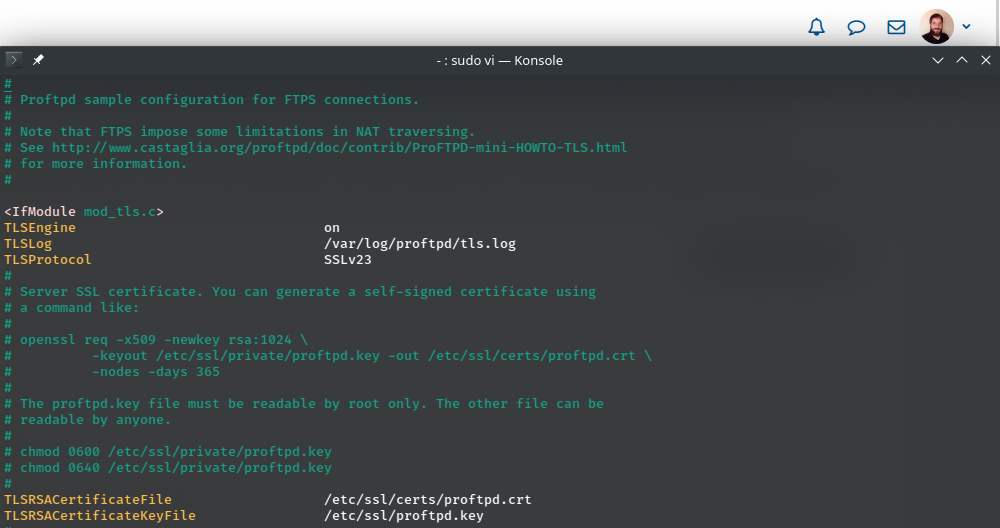
\includegraphics[scale=0.50]{tsl-4.png}
    \caption{Fichero tsl.conf modificado}
\end{figure}

Por último, hemos intentado conectar al servidor con el comando \textbf{ftp}, como hemos hecho hasta ahora, pero este
comando no soporta SSL por lo que el servidor no nos ha dejado conectar como podemos ver en la siguiente captura.

\begin{figure}[H]
    \centering
    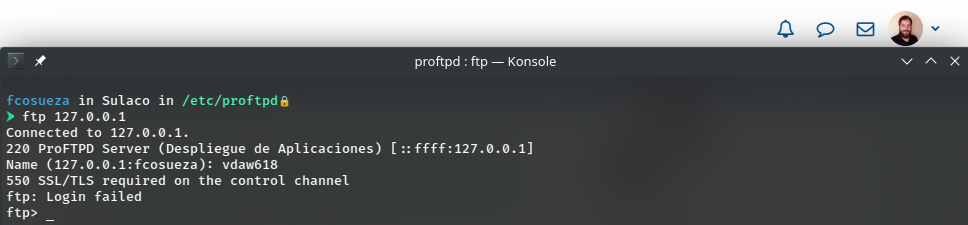
\includegraphics[scale=0.50]{tsl-5.png}
    \caption{Conexión denegada con el comando ftp}
\end{figure}

Para realizar la conexión correctamente, en el siguiente ejercicio emplearemos un cliente que lo soporte, en concreto, Filezilla.

\subsection{Ejercicio 5: Instalación y configuración de un cliente gráfico FTP}
Ahora que ya hemos instalado el servidor FTP vamos a instalar y configurar un cliente gráfico FTP que acceda a los servicios desplegados en el ejercicio anterior. Para ello deberás realizar lo siguiente:
\begin{itemize}
    \item Instala a través del gestor de paquetes de Ubuntu, el cliente gráfico de \textbf{FTP Filezilla}, documentando adecuadamente el proceso.
    \item Configura un perfil en el gestor de sitios de Filezilla para el \textbf{acceso anónimo al servidor FTP} que has configurado en la actividad 2 y comprueba que te puedes conectar, y que no te permite subir ficheros ni borrar el que hay.
    \item Configura un perfil en el gestor de sitios de Filezilla para el acceso al servidor FTP mediante el usuario virtual que has configurado en la actividad 3 y comprueba que te puedes conectar, y que te permite subir ficheros.
    \item Documenta adecuadamente el proceso.
\end{itemize}

\subsubsection{Solución}
En este ejercicio vamos a instalar el cliente de FTP \textbf{FilleZilla}, que nos permitirá conectar al servidor FTP con diferentes usuarios, así como realizar una conexión segura con este.

En primer lugar hemos intentado instalar \textbf{Filezilla}, y digo hemos intentado porque cuando hemos ido a instalarlo resulta que ya estaba instalado. Independientemente de ésto, la instalación de puede realizar desde los repositorios oficiales de Ubuntu, usando APT. En la siguiente captura vemos al ejecución del comando en una terminal.

\begin{figure}[H]
    \centering
    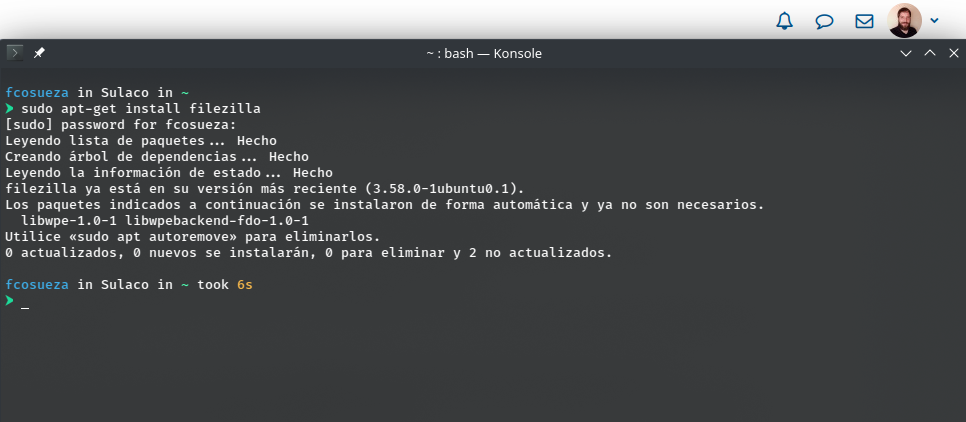
\includegraphics[scale=0.50]{filezila-1.png}
    \caption{Instalación de Filezilla}
\end{figure}

El siguiente paso ha sido realizar una conexión anónima al servidor y comprobar que no nos permite subir ni eliminar archivos. Filezilla ya tiene por defecto activada la conexión TLS por lo que solo hemos tenido que introducir los datos en del servidor y el nombre de usuario, en nuestro caso \textbf{127.0.0.1} y \textbf{anonymous} respectivamente, y realizar la conexión rápida, como vemos en la siguiente captura.

\begin{figure}[H]
    \centering
    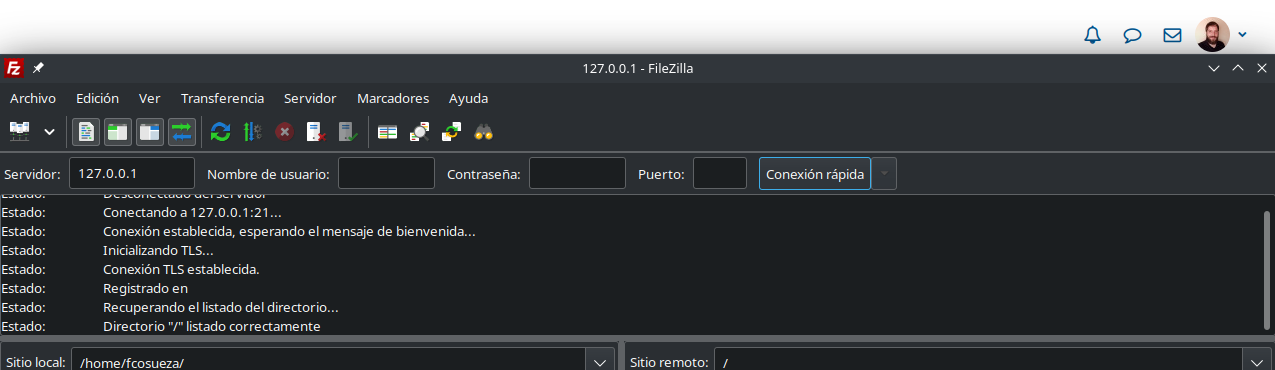
\includegraphics[scale=0.50]{filezila-2.png}
    \caption{Conexión anónima con Filezilla}
\end{figure}

A continuación hemos intentado subir un archivo, pero como podemos ver en al siguiente captura, la operación no esta permitida para este usuario por lo que no hemos podido realizarla. es lo esperado, ya este usuario no tiene dichos permisos.

\begin{figure}[H]
    \centering
    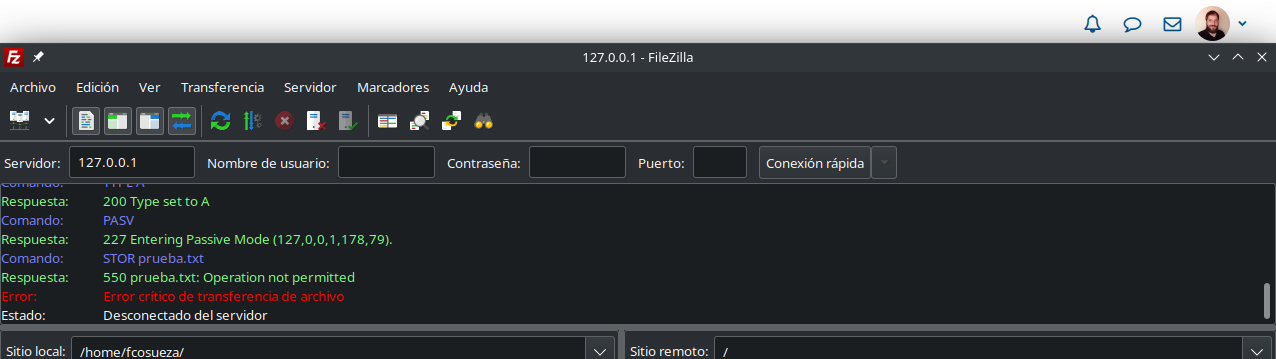
\includegraphics[scale=0.50]{filezila-3.png}
    \caption{Intento de subida de archivo con el usuario anónimo}
\end{figure}

Ahora vamos a conectar con el usuario virtual que hemos creado. El proceso es el mismo que en anterior caso, con la diferencia de que cambiamos los credenciales, insertando el usuario creado (vdaw168) y su contraseña (prueba). Además, en este caso, si nos ha permitido realizar la subida, ya que este usuario si tiene permisos, como podemos ver en la siguiente captura.

\begin{figure}[H]
    \centering
    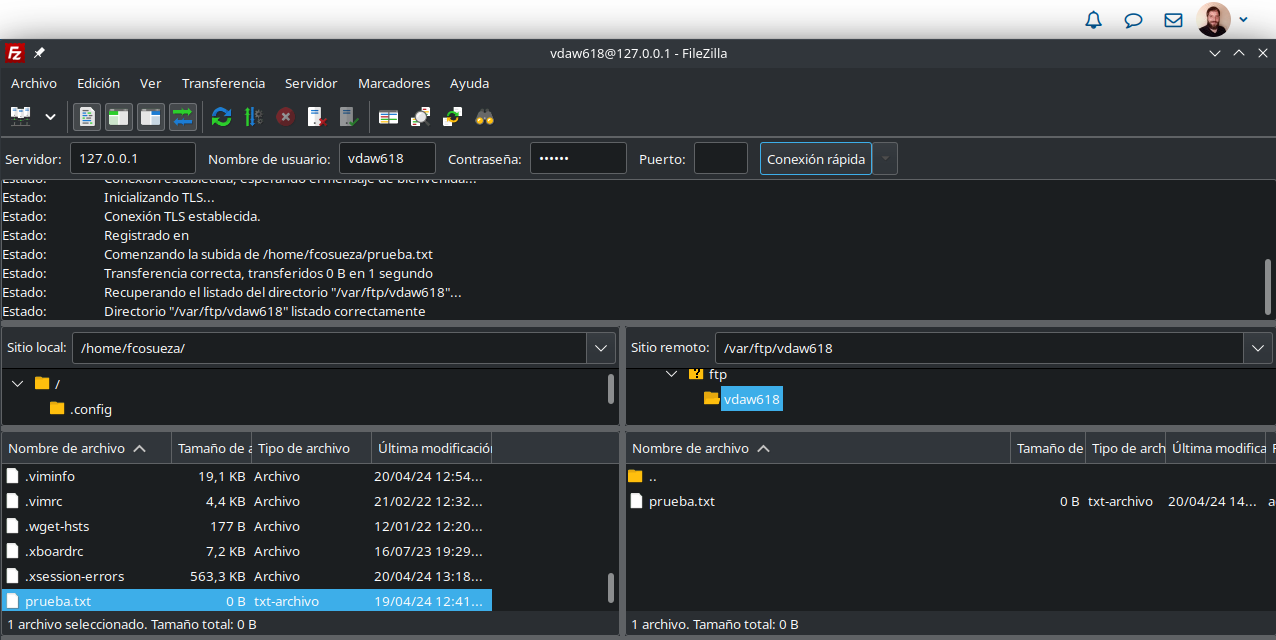
\includegraphics[scale=0.50]{filezila-4.png}
    \caption{Conexión con el usuario vdaw168 y subida del archivo}
\end{figure}

\subsection{Ejercicio 6: Uso de un navegador como cliente FTP}
Aunque por motivos de seguridad, la mayoría de los navegadores ya no permiten su uso como clientes FTP, aún es posible hacerlo utilizando navegadores obsoletos o incluso el explorador de archivos de Windows. En esta actividad utilizaremos la primera opción (Si usas una versión 18 de Ubuntu y no has actualizado el navegador Firefox también te puede servir):

\begin{itemize}
    \item Descarga una versión portable de Mozilla Firefox (70 o anterior).
    \item Ahora accede con tu usuario de sistema o con tu usuario virtual.
    \item Comprueba que tienes acceso a los ficheros y carpetas correspondientes a ese usuario.
    \item Documenta adecuadamente el proceso.
\end{itemize}

\subsubsection{Solución}
En este ejercicio vamos a acceder al FTP usando un navegador. En este caso, se ha usado el navegador propio de KDE, \textbf{Konqueror}, ya que es de los pocos navegadores actuales que soportan FTP.

En el enunciado se dice que se use alguna versión obsoleta de Firefox, pero ha sido imposible hacerlas funcionar en la versión 22.04 de Kubuntu, ya que la última versión con soporte para FTP es la versión 90.0 de Firefox, donde se puede habilitar en la configuración y desde esa versión el sistema de comunicación de Ubuntu ha sido modificado. Así que se ha optado por la opción de utilizar un navegador, actual y funcional que aún soporta el protocolo FTP.

Para conectar al FTP desde el navegador, solo tenemos que introducir en la barra de direcciones la dirección \textbf{\textit{ftp://127.0.0.1}}. Esto nos abrirá una ventana donde nos permitirá introducir el usuario y contraseña. Nosotros hemos introducido el usuario virtual creado, como podemos ver en la siguiente captura.

\begin{figure}[H]
    \centering
    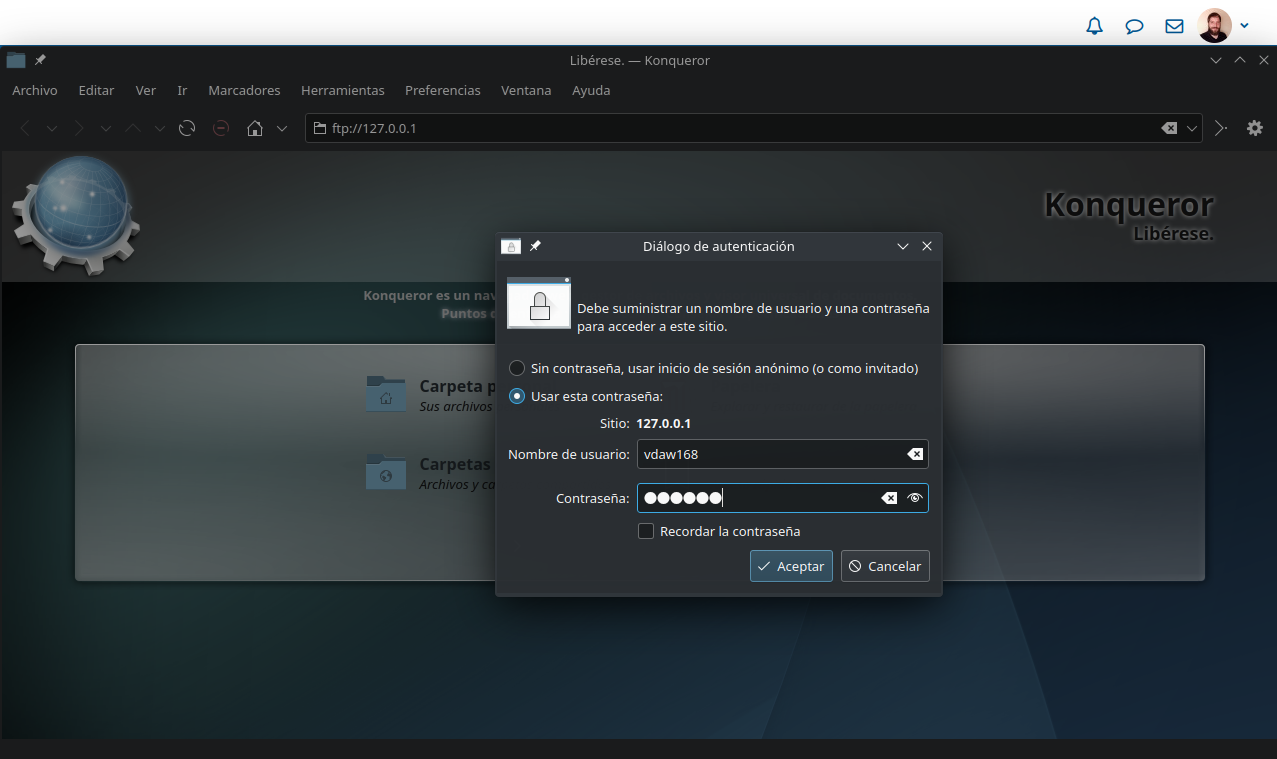
\includegraphics[scale=0.50]{firefox-1.png}
    \caption{Inicio de sesión desde el navegador Konqueror}
\end{figure}

Con la configuración actual del servidor nos encontramos con un problema, y es que no nos dejará conectar ya que requiere soporte para TLS. Así que la opción que nos queda es deshabilitar temporalmente el soporte para TLS en el servidor, lo que se ha realizado comentando la opción \textbf{LoadModule mod\_tls.c} en el archivo \textbf{modules.conf} de ProFTPd.

Una vez realizado esto, se ha introducido la dirección \textbf{ftp://vdaw618@127.0.0.1}, donde indicamos el usuario con el que queremos conectar, y se ha realizado la conexión. Como podemos ver en la siguiente captura, nos ha cargado el directorio raíz de este usuario permitiéndonos además, crear o eliminar archivos, como se ve en la siguiente captura.
\begin{figure}[H]
    \centering
    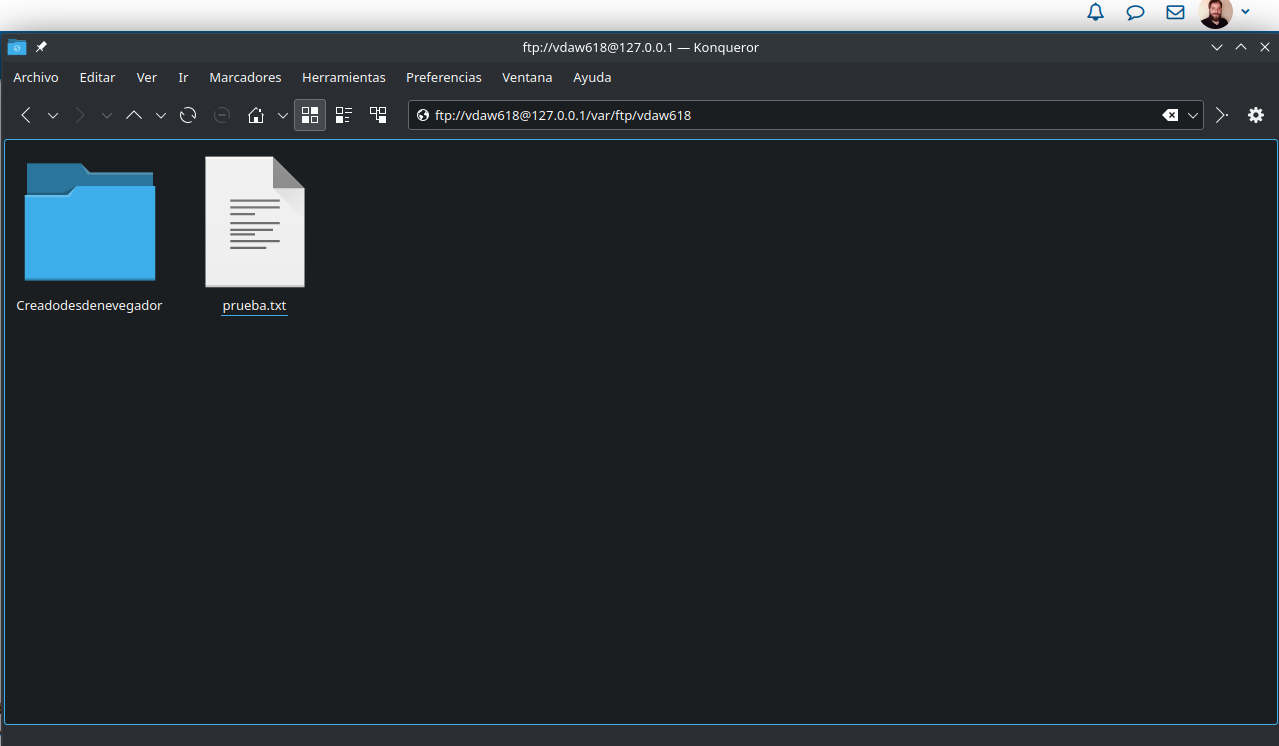
\includegraphics[scale=0.50]{firefox-2.png}
    \caption{Acceso a la carpeta del usuario vdaw618 desde el navegador}
\end{figure}

\subsection{Ejercicio 8: Configuración del servicio FTP en modo activo o pasivo}
Revisa la configuración de tu servidor FTP y comprueba si está configurado en modo activo o pasivo. En caso de que está en modo activo indica qué pasos deberíamos seguir para configurarlo en modo pasivo. ¿Qué modo de funcionamiento es más seguro? Explica tu respuesta.

\subsubsection{Solución}
\textbf{ProFTPd} acepta tanto conexiones en modo pasivo como activo \textbf{por defecto}. Que la conexión se establezca de un modo u otro, como se especifica en el \textbf{RFC 959}, depende del tipo de conexión que solicite, ya sea mediante el comando \textbf{PORT}, para conexiones activas o el comando \textbf{PASV} para conexiones pasivas. Dentro de la configuración de ProFTPd podemos cambiar algunos valores, como puede ser el rango de puertos que queremos usar para las conexiones pasivas, con la directiva \textbf{PassivePorts}.

Si queremos, se podrían limitar los comandos que acepta el servidor, para forzar conexiones de un tipo u otro podemos usar la directiva \textbf{Limit} para bloquear las transferencias activas o pasivas como podemos ver en la \href{http://www.proftpd.org/docs/howto/Limit.html}{docuentación de ProFTPd}. Para ello, podemos limitar los comandos PORT o PASV según nos convenga, como podemos ver en el siguiente código.

\begin{figure}[H]
    \begin{tcolorbox}[sharp corners, colback=yellow!30, colframe=white!20]
        \scriptsize
        \begin{verbatim}
Para limitar el modo activo:

<Limit EPRT PORT>
    DenyAll
</Limit>

Para limitar el modo pasivo:

<Limit EPSV PASV>
    DenyAll
</Limit>
        \end{verbatim}
    \end{tcolorbox}
    \caption{Bloqueo de comando PORT o PASV en ProFTPd}
\end{figure}

Respecto a la \textbf{seguridad de cada modo}, cada uno tiene sus puntos fuertes o débiles, aunque se podría decir que el \textbf{modo activo} es mas seguro, ya que el \textbf{modo pasivo} nos obliga a tener un rango de puertos fuera del firewall en el servidor para que se realice la transferencia de datos.



% Bibliography

%\newpage
%\bibliography{citas}
%\bibliographystyle{unsrt}

\end{document}